\chapter{Definitions}
\label{def}

Following are several concepts related to the problem at hand. These terms will be later referenced in the model section (section \ref{matmod})6.

\section{Introduction}

\begin{figure}
	\centering
		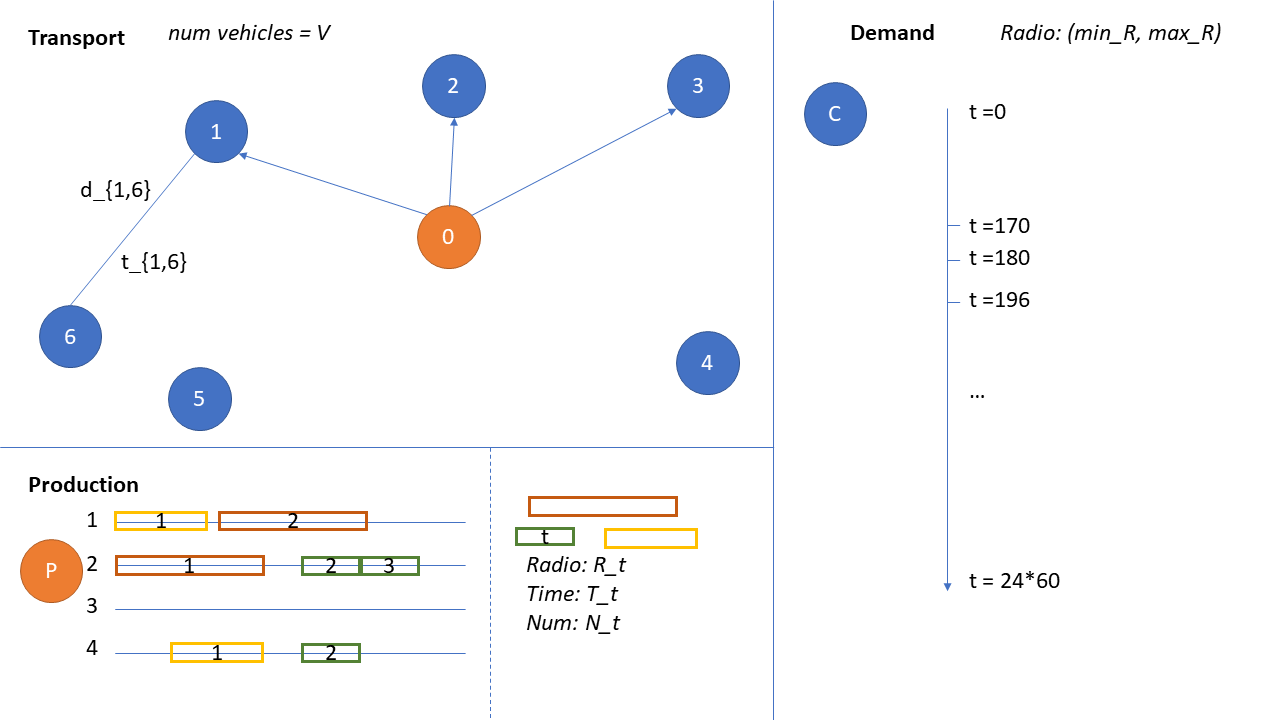
\includegraphics[width=\textwidth]{imagenes/definitions.png}
	\caption{Main definitions}
	\label{fig:definitions}
\end{figure}

Figure \ref{fig:definitions} shows the structure of some of the parameters used in the formulation of the problem. Both the definition and the Mathematical formulation are classified into the three scopes: "`Transport"', "`Demand"', "`Production"'.

The production node "`P"' or "`0"' in orange. Each pair of nodes has a symmetric time and distance.

Demand, for each on of the 6+1 centers "`C"' in is a list of times when a patient needs a dosage, knowing that the radioactivity of the dosage needs to be in a given range.

The production taking place in the node can be done in each production line {1, 2, 3, 4}.
The production is done in batches (or jobs). These jobs can be of one of a set of job types. Each job type has specific characteristics and is represented by a color.

\section{Production}

\subsection{Production line and type}
\label{def:lines}

A production line consists on each of the places where production can happened. Each line works independently from the other an are identical in their capacity to produce.

They have an associated cost to be used at least once during the day.

There exists a definite set of production "`drives"' that a line can be in. They have been called "`production types"'. Each type consists on a combination of three parameters:

\begin{itemize}
	\item Time to produce.
	\item Number of dosages to produce.
	\item Radioactivity level of dosages when produced.
\end{itemize}

Each line can produce any of these production types and can change from producing one type to producing the other without any extra cost.

\subsection{Production job}

A production job consists of a given batch of dosages produced at a specific production line.

It is represented by a tuple with numbers. The first one is the production line it belongs, the second is a correlative number.

Jobs are defined in advance so that each production line has a number of candidate jobs available to potentially use.

Also, each job needs to have assigned a "job type" (see \ref{def:lines} for more information).

\section{Transport}

\subsection{Vehicle}

A vehicle is the means for transporting dosages between the production node and each of the centers. They need to do specific routes between each center in order to arrive on time for each patient's appointment.

There is a finite number of vehicles, all identical. There is no capacity limit on the amount of dosages each vehicle can take in total and the the cost of the vehicle has three components:

\begin{itemize}
	\item Total distance traveled.
	\item Total time traveled.
	\item Usage of vehicle.
\end{itemize}

\subsection{Route}
\label{def:route}

A route is the specific travel of a single vehicle.

It is defined by a tuple with two numbers. The first one is the vehicle that can do the route, the second one is the correlative number of route of that specific vehicle.

Routes are pre-calculated, so each vehicle has the following information:

\begin{itemize}
	\item The number of routes it can do.
	\item The centers the route has to visit, in case of being activated.
\end{itemize}


\section{Demand}

\subsection{Center}

Each center is a physical place where dosages are consumed during the day. There are both distances and times between each center. These distance and times matrices are considered to be symmetrical.

Each center has, in addition, a specific time to unload the dosages once the vehicle arrives.

During the model formulation, centers can also be called nodes.

\subsection{Appointments}

An appointment is 1 dosage administered at a specific time in a specific center.

It is defined as a tuple of two numbers. The first one is the center to which the appointment belongs, the second one is the correlative number of appointment in the day.

The radioactivity in the dosage degenerates with time after production and should be in a specific range when administered to during the appointment.

Patients are groups of appointments and are defined in \ref{sec:patients}.

\subsection{Radioactivity}

\begin{figure}
	\centering
	
		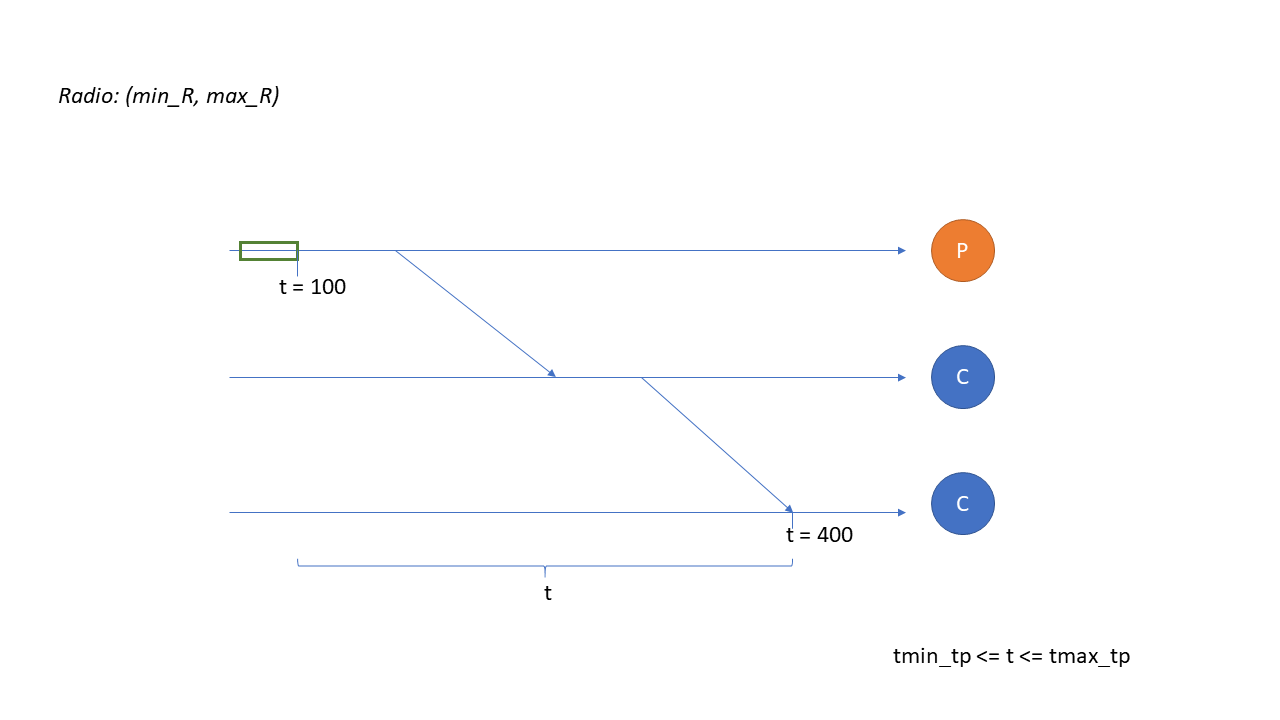
\includegraphics[width=0.80\textwidth]{imagenes/radioactivity.png}
	\caption{Radioactivity time}
	\label{fig:radioactivity}
\end{figure}


The radioactive content of the dosage needs to be calculated based on the ending time of the job that produced it and the moment the patient receives the dosage.

Figure \ref{fig:radioactivity} shows how the dosage moves from the production node, after it is produced, and reaches the patient's center. The time it took the dosage to reach the patient (not the center) is the correct time to measure the radioactivity.

\section{Clustering}

As an important part of the modelization, different groups or clusters have been created. The aim has been to reduce the problem size into one that can be solved by a good mixed integer solver.

As part of these model simplifications, optimality of the objective function has been sacrificed. The idea has been to try to not loose too much quality in the solutions while at the same time trying to help the solvers arrive at near optimal solutions for the simplified problem.


More information on the obtained results, experiments with variations of clusterings and differnet solvers can be found in \ref{results}.


\subsection{Clustering of centers}
\label{def:cluster}

Due to the number of combinations of possible routes (see section \ref{def:route}) that any vehicle can do, centers have been grouped into groups (or clusters).

The clustering of centers has been achieved with a K-means algorithm using the distance matrix between centers. The production center has not been included in the clustering procedure given that this center will be included in every cluster.

\subsection{Cluster-route}

In order to assign groups of centers to vehicles, a clustering of centers has been made. The number of clusters depends on the total number of vehicles and centers available. See section \ref{def:cluster}.

Each route, when active, needs to visit each one of the centers in the cluster. In a sense, it behaves similarly to a Travelling Salesman Problem with time windows.

Given the clustering of centers explained in section \ref{def:cluster}, not all vehicles can visit all centers. Dependind on the configuration adopted and the number of vehicles and centers, each vehicle will be able to visit between 1 and 3 clusters. 

Furthermore, each specific route of a vehicle (see section \ref{def:route}) will only be able to visit 1 cluster. The idea is to have many different vehicles capable of servicing the same cluster. This way it is possible to reduce the number of vehicles if necessary without compromising feasibility.

\subsection{Clustering Job-Job types}

In order to reduce the size of the problem and break the symetry on the decision variables, each production line can produce only certain types of jobs. For example, the first production line can produce only the first two types of jobs.

We thus sacrifice optimality (we reduce some possibilities) in order not to have too many decision variables.

The maximum number of jobs per line also depends on which types of jobs the line can do. It is assumed that a line that only has particularly long-duration job types available will not do many jobs.

\subsection{Patients as clusterings of appointments}
\label{sec:patients}

On one hand appointments happen at arbitrary moments during the idea. On the other hand the radioactivity is calculated each 30 minutes. This means that grouping appointments inside a 30 minute period or a period that is a multiple of 30 minutes is reasonable to attempt.

Thus, we define a patient as a number of dosages that need to be administered between a minimum and a maximum time. The minimum and maximum times are used to be able to guarantee that the dosage will reach with the correct radioactivity for every appointment inside the range and be sure the route will arrive before the minimum time.

A particular case of this formulation would be to treat each appointment as a patient. In this case, the patient would have a dosage of 1 and a minimum time equal to the maximum time.

\subsection{Example}

\begin{figure}
	\centering	
		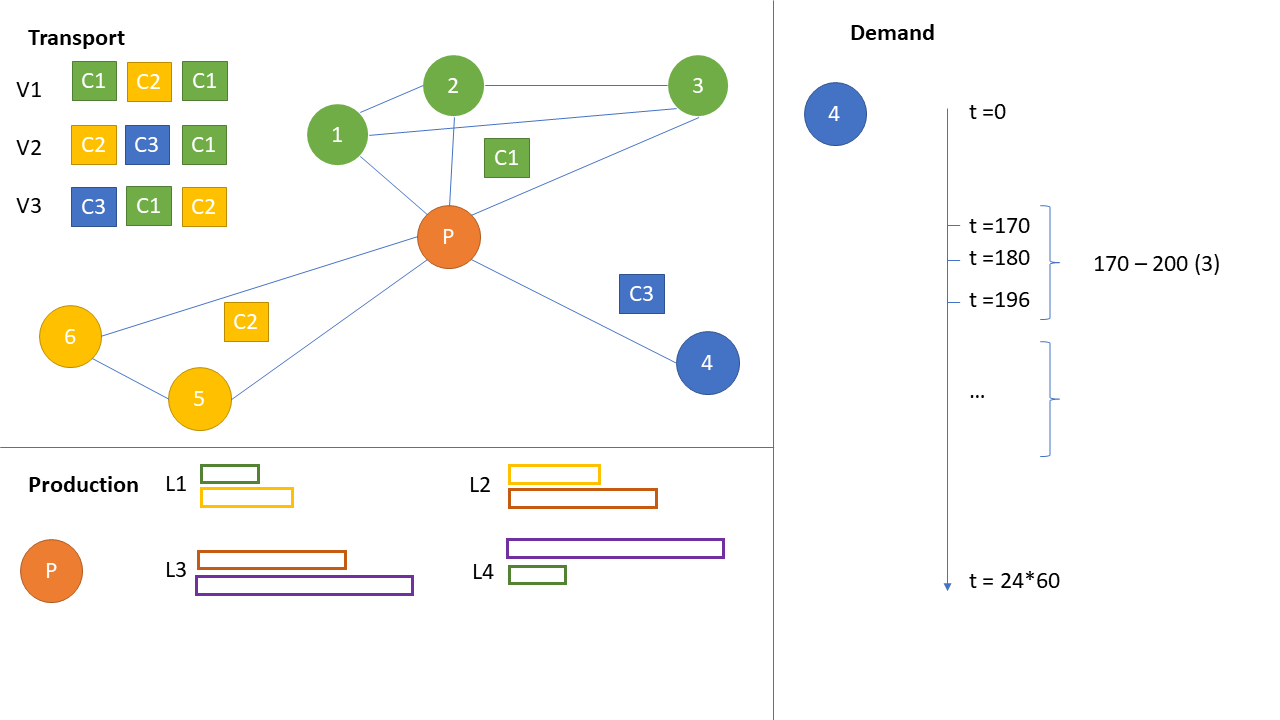
\includegraphics[width=\textwidth]{imagenes/clustering.png}
	\caption{Clustering example}
	\label{fig:clustering}
\end{figure}


The figure \ref{fig:clustering} shows an example of each type of clustering. 


In the case of transport, it shows with a different color a possible grouping of centers into clusters "`C1"' to "`C3"'. In addition to that it's shown an example of routes done by each of three vehicles. Vehicle one made routes to clusters "`C1"', "`C2"' and then "`C1"' again. This means that three routes were done by each vehicle.


In the case of production it shows the possible job types that each line can do: line 1 can only do job types corresponding to color "`yellow"' and "`green"' and so forth.


Finally, in the case of demand, three appointments on center 4 have been grouped into a patient with three dosages between minutes 170 and 196 of the day.

